\documentclass{amia}
\usepackage{graphicx}
\usepackage[labelfont=bf]{caption}
\usepackage[superscript,nomove]{cite}
\usepackage{color}
\usepackage{multirow}

\begin{document}

\title{Predicting Success of Clinical Interviews via Probabilistic Modeling of Patient-Provider Communication Sequences}

\author{Mehedi Hasan, BS$^{1}$, Alexander Kotov, PhD$^{1}$, April Carcone, PhD$^{2}$, Mind Dong, PhD$^{1}$, Sylvie Naar, PhD$^{2}$}

\institutes{
$^1$Department of Computer Science,  
$^2$Pediatric Prevention Research Center, Wayne State University, Detroit, Michigan\\
}

\maketitle

\noindent{\bf Abstract}
\textit{The problem of analyzing temporally ordered sequences of past events to make predictions related to the observed sequence of events arises in many data analytics scenarios in healthcare informatics. In this paper, we focus on automating the analysis of patient-provider communication sequences in the context of clinical interviews and propose the methods for identifying the most effective communication exchanges to elicit a particular type of patient response and dynamically predicting this type of response in an observed patient-provider communication. Our proposed method for predicting the likelihood of desired patient behavioral response in communication sequences can be used in conjunction with either Markov Chain or Hidden Markov Model and can significantly decrease the effort  required to develop effective interventions to address many public health conditions, such as childhood obesity. It achieved 75.32\% and 79.89\% F-measure for normal sequences and 97.36\% and 96.99\% F-measure for alternate sequences using first and second order Markov Chain and Hidden Markov Model, respectively,  to model communication sequences. Our results indicate that individual short length patient-provider communication sequences are highly indicative of the overall progression and future trajectory of a clinical interview and can be used to predict its overall success. Our results have broad implications for qualitative public health research by providing a formal mechanism to facilitate the development of effective behavioral interventions.}

\section*{Introduction}
Data in the form of temporally ordered sequences of discrete or continuous observations (e.g., symbolic sequences such as notes in patient EHR, diagnostic codes, protein or DNA sequences or continuous time series, such as ECG measurements) arise in various domains of health informatics. The order of observations in a sequence is challenging to capture using features, which makes sequence classification a more challenging task than traditional classification. In general, sequence classification methods can be divided into three  categories: feature-based, distance metric-based and model-based method. Feature-based classification methods transform a sequence into a feature vector and apply a standard supervised learning algorithm, such as support vector machine \cite{leslie2004fast} or decision tree \cite{chuzhanova1998feature}. Shapelet \cite{ye2009time} and pattern \cite{kudenko1998feature, lesh1999mining} based techniques as well as hierarchical approaches \cite{nallam2016effective} have been proposed instead of standard classifiers as well. Distance-based methods measure the similarity between sequences to determine the quality of classification. The most commonly used distance function is Euclidian distance \cite{keogh2003need} with Dynamic Time Wrapping \cite{keogh2000scaling} used for more flexible matching in time series data. The third type of sequence classification methods, first create a probabilistic model of a sequence, such as Hidden Markov Model \cite{rabiner1989tutorial} (HMM).

Sequence classification has a broad range of real word applications from genomics and health informatics to finance and anomaly detection. In genomics research, sequence classification is widely used to classify protein and text sequence data \cite{yakhnenko2005discriminatively} and detect the function of new proteins \cite{deshpande2002evaluation}. In health informatics, ECG measurements are considered as multi-dimensional time series and are used to classify individuals as healthy or having a heart disease \cite{wei2006semi}. Sequence classification is also used for anomaly detection such as abnormal access to systems \cite{lane1999temporal} and malware \cite{drew2017polymorphic}.    

In this paper, we direct our focus towards patient-provider communication sequences in the context of clinical interviews. Specifically, we focus on the transcripts of Motivational Interviews (MI) with obese adolescents and their caregivers. Childhood obesity is a serious public health concern in the United States and worldwide. Recent estimates indicate that approximately one third (31.8\%) of US children age 2-19 years are overweight and 16.9\% are obese \cite{ogden2012prevalence}. Adolescents who are obese likely continue to be obese in adulthood and have a greater risk of heart disease, type 2 diabetes, stroke, cancer, and osteoarthritis \cite{general2010surgeon}. One approach to designing an effective obesity intervention is Motivational Interviewing, an evidence-based counseling technique to increase intrinsic motivation and self-efficacy for health-related behavior change. The goal of MI counseling session is to encourage patients to explore their own desires, ability, reasons, need for and commitment to the targeted behavior change. These statements, referred to as ``change talk'' (or CT), consistently predict actual behavior change that can be sustained for as long as 34 months after an interview. However, the ability of counselors to consistently elicit this type of patient communication requires knowledge of effective communication strategies for a variety of patients, which can only be obtained through analysis of a large number of annotated interviews. Since manual annotation and examination of transcripts is a very time-consuming process, development of new obesity interventions can take years. Therefore, there is a need for informatics-based methods to facilitate the development of effective MI-based interventions. 

While our previous work \cite{kotov2015interpretable, hasan2016study} explored several machine learning methods for automatic annotation of clinical interview fragments with a specialized codebook containing 115 patient and provider behavior codes \cite{carcone2013provider}, in the work, we propose probabilistic methods to identify patient-provider communication sequences that are likely to elicit the desired patient behavioral response (i.e. change talk or commitment language) and to dynamically estimate the likelihood of observing this desired response at any point during a clinical interview based on all coded previous patient-provider communication exchanges in the same interview.

While sequential analysis \cite{eide2004physician} was performed on physician-patient dialogue to establish the relationship between physician and patient behaviors associated with patients' exhibiting cues, there have been only a handful of previous studies on modeling annotated sequences of patient-provider communication exchanges and predicting a desired patient behavior in the context of clinical interviews.   

\section*{Methods}
\subsection*{\textit{Data collection}}
The experimental dataset for this work was constructed from the transcripts of 37 motivational interviews, which include a total of 11,353 segmented and annotated utterances. Each motivational interview consists of counselor-adolescent and counselor-caregiver sessions. Since the ultimate goal of a motivational interview is to increase the desire and ability of adolescents for a targeted behavior change, we considered only communication sequences from counselor-adolescent sessions and disregarded all communication sequences from counselor-caregiver sessions. The utterances were annotated based on MYSCOPE codebook \cite{carcone2013provider} with 115 distinct behavior codes, which are grouped into the youth, caregiver, and counselor code groups. Utterances were divided into successful and unsuccessful communication sequences. Successful communication sequences result in either positive change talk or commitment language statements by an adolescent, while unsuccessful sequences are the ones that result in negative change talk, negative commitment language or the ones in which neither change talk nor commitment language statements occur. Out of 1072 observed sequences, 880 were positive and 192 were negative. Alternate sequences are the possible combination of a normal sequence where two consecutive utterances cannot belong to the same speaker. For example, there are 6 possible alternate sequences ({C1, A1, C2, A3}, {C1, A1, C3, A3}, {C1, A1, C4, A3}, {C1, A2, C2, A3}, {C1, A2, C3, A3} and {C1, A2, C4, A3}) for the normal sequence {C1, A1, A2, C2, C3, C4, A3}, where adolescent and counselor codes are represented by A and C, respectively. A total of 18753 alternate sequences have been observed, out of which 18139 were successful and 614 were unsuccessful ones. For each type of sequence (normal and alternate), one probabilistic model was trained using successful sequences and one model was train using unsuccessful sequences. Statistics of experimental dataset are presented in Table~\ref{tab:data_dist} and a fragment of an adolescent session transcript is presented in Table~\ref{tab:anno_examp}. \\

\begin{table}[h]
\centering
\caption{Statistics of experimental dataset.}
\label{tab:data_dist}
  \begin{tabular}{|l|l|l|l|l|l|}
  \hline
   \textbf{Sequence type} & \textbf{Total sequences}  & \textbf{\# Successful sequences}  & \textbf{\# Unsuccessful sequences} & \textbf{Avg. length} \\ \hline      
 Normal sequences & 1072 & 880 (82.09\%) & 192 (17.91\%) & 5.83 \\\hline
Alternate sequences & 18753 & 18139 (96.72\%) & 614 (3.28\%) & 12.89 \\\hline 
  \end{tabular}
\end{table} 

Annotation column in Table~\ref{tab:anno_examp} shows the sequence of behavior codes from top to bottom, where counselor starts with an open-ended question and gets positive feedback at the end. \\

\begin{table}[h]
\caption{Fragment of the annotated transcript of a dialogue between a counselor and an adolescent.}    
\label{tab:anno_examp}
\centering
\begin{tabular}{|l|p{3.6cm}|l|p{8cm}|}
\hline
Annotation  & Description & Speaker & Text \\\hline
331 &	Open-ended question, elicit change talk positive &	Counselor &	do you feel like making healthier choices for your snacks and your meals is something you would be able to do? mm-hmm meaning is that food available for you? \\\hline
117 &	Low Uptake, positive	& Adolescent &	Yes \\\hline
301 &	Structure Session	& Counselor &	okay and thats an important thing for us to think about cause i would not want to help you come up with a plan that you would not be able to do without somebody else help so the last part of your plan is how somebody could be supportive to you meaning how they can help you be successful and so we should choose somebody who you feel like is around often enough \\\hline
112 &	Change Talk positive	& Adolescent &	my um aunt \\\hline
301 &	Structure Session	& Counselor &	okay so lets stick something my aunt can do \\\hline
112 &	Change Talk positive &	Adolescent &	she could when i am doing when i am eating something that i should i could not be eating but so i can choose something healthy she could tell me not to eat it \\\hline
309 &	Affirm, low &	Counselor &	okay that sounds like a really great suggestion \\\hline
\end{tabular}
\end{table}  

\subsection*{\textit{Sequence classification techniques}}

Generally, a sequence is a temporally ordered set of events. In our study, an event is a behavior code represented as a symbolic value, such as 117 (low uptake, positive), 331 (open-ended question), etc.  Given a sequence of behavior codes represented as $S_i = \{x_1, x_2,...,x_n\}$ and a set of class labels $L = \{l_1, l_2,...,l_m\}$, the task of sequence classification is to learn a sequence classifier C, which is a function mapping a sequence $S_i$ to a class label $l_i \in L$, written as, $C : S_i \to l_i, l_i \in L$, where $L$ is fixed and known in advance. In our case, the labels are ``successful'' and ``unsuccessful'' (motivational interview).

We model successful and unsuccessful patient-provider interactions using first- and second-order Markov Chain (MC) and Hidden Markov Model (HMM), which are probabilistic methods for modeling discrete observation sequences with finite vocabulary. Although HMM was originally developed for speech recognition \cite{rabiner1989tutorial}, it is one of the most widely used methods for sequence modeling \cite{mutsam2016maximum, eickeler1998hidden, srivastava2007hmm, won2004training, chai2001folk}.

\textbf {Markov Chain}: In probability theory, a Markov model \cite{} is a stochastic model used to model randomly changing systems where it is assumed that future states depend only on the present state and not on the sequence of events that preceded it (that is, it assumes the Markov property). Generally, this assumption enables reasoning and computation with the model that would otherwise be intractable. For the sequential analysis, we built two Markov models $M$ and $\overline{M}$ describing provider strategies and patient responses in case of successful ($M$) and unsuccessful ($\overline{M}$) motivational interviews. A Markov model $M$ can be represented as a weighted directed graph $G = (V, E, p)$, in which:

\begin{itemize}
\item $V = \{CML+, CHT+, CHT-, T-AMB, CCT, BLT, LUP+, LUP-, HUP-W, ...\}$ is a set of vertices, consisting of adolescent and counselor MI behavior codes;
\item $E \subseteq V \times V$ is a set of edges corresponding to posssible transitions from one MI behavior code to the other in a sequence;
\item $p_M:E\rightarrow[0...1]$ is a function that assigns probability $p(c_i|c_j)$ to an edge between the MI behavior codes $c_i$ and $c_j$ based on maximum likelihood estimator:

\begin{equation}
P_M(c_j|c_i) = \frac{n_{c_i,c_j}}{n_{c_i}}
\end{equation}

\end{itemize}

where $n_{c_i,c_j}$ and $n_{c_i}$ are the number of times a transition between the MI behavior codes $c_i$ and $c_j$ and the code $c_i$ has been observed in the training data. Given a Markov model $M$ (such that $S\subseteq V$), the probability that a sequence of MI behavior codes $S = \{C_1,...,C_N\}$ has been generated from a Markov model $M$ is:

\begin{equation}
P_M(S) = \prod_{i=2}^N p_M(c_i|c_1,\dots,c_{i-1})=\prod_{i=2}^N p_M(c_i|c_{i-1})
\end{equation}

The likelihood of success of a given motivational interview at a given time point, given a sequence of MI behavior codes observed prior to that point, is estimated based on the following formula:

\begin{equation}
p(S\rightarrow CML+) = \log\left(\frac{P_M(S)}{P_{\overline M}(S)}\right)= \sum_{i=2}^N p_M(c_i|c_{i-1})-\sum_{i=2}^N p_{\overline M}(c_i|c_{i-1})\label{eq:class}
\end{equation}

if $p(S\rightarrow CML+) > \delta $, where $\delta$ is an empirically determined threshold, the interview is predicted to result in positive change talk or commitment language. Estimating the model on the training data involves experimentally determining the value of $\delta$, resulting in the highest prediction F-measure with lower bias. Figure~\ref{fig:delta} illustrates the accuracy of Markov model-based method by varying the value of $\delta$. As can be seen from Figure~\ref{fig:delta}, F-measure varies insignificantly, when $\delta $ is between -5 to -1, due to possible bias. However, F-score sharply decreases after $\delta = -0.9$. Thus, -0.9 is the optimal value of $\delta $, where F-measure is the highest with lower bias. 

\begin{figure}[htb!]
    \centering
    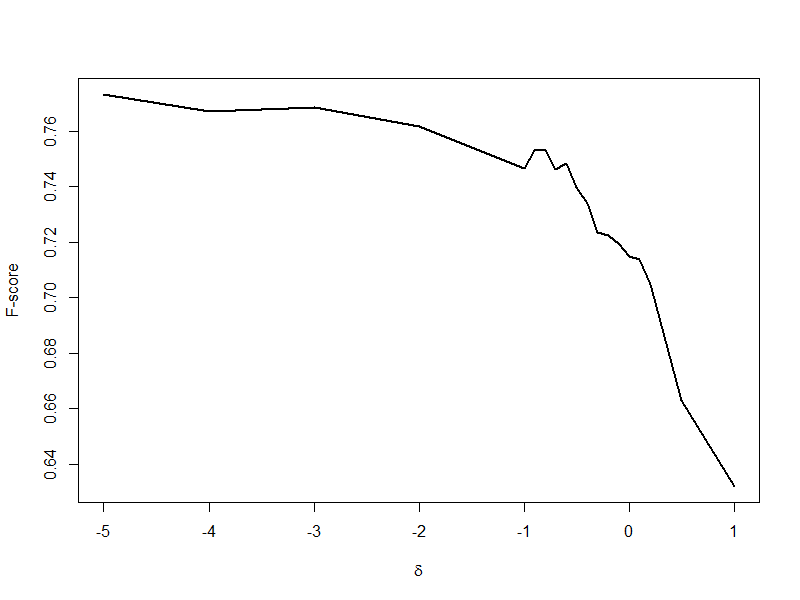
\includegraphics[width=0.70\textwidth]{figures/delta.png}
    \caption{\textbf{Accuracy of the proposed Markov model-based method by varying the value of $\delta$}.}
    \label{fig:delta}
\end{figure}

The Markov model we have discussed so far is referred to as the first-order MC, since it only considers immediately preceding behavior code to compute the state transition probability matrix. A generalization of the first-order MC is the $k^{th}$ order MC, in which the transition probability to a particular state (symbol) $x_i$ is computed by looking at the k preceding states (symbols). Thus, $k^{th}$ order Markov chain will have $N^{k}$ states each associated with a sequence of k symbols. In our experiment, we also used second order Markov model. Hence, our model has $N^2$ states with transition probability matrix of size $N^2 \times N$.  

\textbf {Hidden Markov Model (HMM)} is a powerful tool for statistical modeling of processes varying in time. HMMs are widely used for sequence analysis because of their ability to incorporate dependencies among elements in sequence. HMM can be considered as a doubly embedded stochastic process with a process that is not observable (hidden process) and can only be observed through another stochastic process (observable process) that produces a sequence of observations. An HMM can be fully specified by the following quintuple:

\begin{center}
$\lambda = (N, M, A, B, \pi)$
\end{center}

\begin{itemize}
\item N is a number of hidden states in the model
\item M is a number of distinct observations symbols per state, i.e. the discrete vocabulary size
\item A is an $N\times N$ state transition probability distribution matrix $A = \{a_{ij}\}$
\item B is an $N\times M$ matrix $B = \{b_j(k)\}$ with observation symbol probability distribution for each state 
\item $\pi$ is the initial state distribution vector $\pi = \{\pi_i\}$
\end{itemize}

We exclude the structure parameters M and N to designate HMM using a compact notation:

\begin{center}
$\lambda = (A, B, \pi)$
\end{center} 

The key difference between HMM and MC is that HMM requires specifying the number of hidden states as a model parameter and then the model figures out a sequence of hidden states that best explains the observations along with state transition probabilities and distributions of observation symbols for each state. The Baum-Welch algorithm was used to estimate the parameters of HMMs for successful and unsuccessful interviews using the corresponding training set, while the Viterbi algorithm was used to determine the most likely sequence of hidden states for a given sequence of observations. After assignment of hidden states, the log-likelihood of successful outcome can be estimated using Eq.~\ref{eq:class}. As in the case of MC, we also experimented with second-order HMM.   

\subsection*{\textit{Evaluation methods}}
The performance of classifiers is reported on the basis of 5-fold cross-validation by using weighted macro-averaging over folds. Precision, recall, F-measure and accuracy were used to evaluate the performance of classifiers. A true positive (TP) was counted when classifier correctly classified the sequence into actual class; a false positive (FP) was counted when classifier incorrectly classified other classes to the considered class; a false negative (FN) when the considered class incorrectly classified to other classes. The precision of a class was defined as the ratio between the numbers of correctly classified sequences and all sequences identified as that particular class by the classifier. In other words, Precision = TP / (TP + FP). Recall of a class was defined as the ratio between the numbers of correctly classified sequences and all sequences of that particular class in the gold standard (labeled data set). In more specifically, Recall = TP / (TP + FN). Similarly, Accuracy of a class was also defined as the ratio between the numbers of correctly classified sequences and a total number of sequences for that particular class in the gold standard. However, F-measure can be computed as the harmonic mean of precision and recall, or 2 x Precision x Recall / (Precision + Recall).  

\section*{Results}
Experimental evaluation of the classification of utterance sequences by using the proposed probabilistic models is reported with two set of experiments: the first set of experiment was focused on normal sequences, while the second set of experiment was performed on alternate sequences. 

\subsection*{\textit{Predictive performance for normal PPC code sequences.}}
Performance summary for the classification of normal sequences is presented in Table~\ref{tab:result_norm_seq}. It follows that first-order HMM demonstrates the best performance achieving the highest precision 0.7980 with 0.7989 F-measure. However, second-order Markov Chain demonstrates the lowest performance in terms of precision and F-measure. It can be seen that the lowest recall of 0.7686 is achieved by the first-order MC. On the other hand, second-order HMM achieves the highest recall 0.8449 and accuracy 0.8449. From Table~\ref{tab:result_norm_seq}, it follows that second-order MC and HMM have lower precision and F-measure, but higher recall and accuracy than first-order MC and HMM. Precision and F-measure decrease by 6.74\% and 2.39\%, in case of MC, and by 7.27\% \& 2.09\%, in case of HMM, when going from first- to second-order models. In contrast, recall improves by 3\%--5\%, in case of both MC and HMM, when going from first- to second-order models. Overall, HMM performed better than MC for normal sequences. \\

\begin{table}[h]
\centering
\caption{Performance of MC and HMM for predicting success of normal patient-provider communication sequences. The largest value for each performance metric is highlighted in bold.}
\label{tab:result_norm_seq}
  \begin{tabular}{|l|l|l|l|l|l|}
  \hline
   \textbf{Model} & \textbf{Order}  & \textbf{Precision}  & \textbf{Recall} & \textbf{F-Measure} & \textbf{Accuracy}\\ \hline    
    
 \multirow{2}{*}{General Markov chain} & First order & 0.7387 & 0.7686 & 0.7532 & 0.7686\\\cline{2-6}
 & Second order & 0.6889 & 0.7889 & 0.7352 & 0.7889\\ \hline
 \multirow{2}{*}{Hidden Markov Model} & First order & \textbf{0.7980} & 0.8059 & \textbf{0.7989} & 0.8059\\ \cline{2-6}
 & Second order & 0.7400 & \textbf{0.8449} & 0.7822  & \textbf{0.8449}\\ \hline
 
  \end{tabular}
\end{table} 

\subsection*{\textit{Predictive performance for alternate PPC code sequences}}
Table~\ref{tab:result_alt_seq} shows the classification performance of models applied on alternate sequences. The results demonstrate that second order hidden Markov model performed better than Markov chain in terms of recall and achieved 97.13\% recall. Second order general Markov model shows the highest precision 0.9778 as well as highest F-measure 0.9736. On the other hand, first order hidden Markov model displays the lowest performance in all metrics compared to all other models. It was also examined that every model perform better in second order compared to first order. General Markov chain achieves 0.01\%, 2.72\% and 1.37\% improvement for precision, recall and F-measure, respectively, from first order to second order. Similarly, hidden Markov model achieves 3.32\%, 4.30\% and 4.82\% improvement for precision, recall and F-measure, respectively, from first order to second order. Overall, second order Markov model performs better for alternate utterance sequences. \\

\begin{table}[h]
\centering
\caption{Performance of MC and HMM for predicting success of normal patient-provider communication sequences. The largest value for each performance metric is highlighted in bold.}
\label{tab:result_alt_seq}
  \begin{tabular}{|l|l|l|l|l|l|}
  \hline
   \textbf{Model} & \textbf{Order}  & \textbf{Precision}  & \textbf{Recall} & \textbf{F-Measure} & \textbf{Accuracy}\\ \hline    
    
 \multirow{2}{*}{General Markov chain} & First order & 0.9777 & 0.9437 & 0.9604 & 0.9437\\\cline{2-6}
 & Second order & \textbf{0.9778} & 0.9694 & \textbf{0.9736} & 0.9694\\ \hline
 \multirow{2}{*}{Hidden Markov Model} & First order & 0.9392 & 0.9313 & 0.9253 & 0.9392\\ \cline{2-6}
 & Second order & 0.9704 & \textbf{0.9713} & 0.9699  & \textbf{0.9713}\\ \hline
 
  \end{tabular}
\end{table}

\subsection*{\textit{Common patterns}}
Table~\ref{tab:common_patterns} shows some successful and unsuccessful patterns which appeared more frequently in a motivational interview. It can be seen that most successful patterns start with a summary of the discussion or open-ended or closed-ended question. After that, if adolescent demonstrates positive behavior change, counselor reflect that positive attitude immediately so that adolescent can stick with the decision and show his own desire for positive behavior change. On the other hand, general information of counselor can lead to a negative behavior change of adolescent, while showing a positive attitude in the previous step. Because adolescent changes their topic more frequently when general questions were asked.   

\begin{table}[h]
\centering
\caption{Common patterns in successful and unsuccessful motivational interviews.}
\label{tab:common_patterns}
  \begin{tabular}{|l|l|l|l|l|l|}
  \hline
   \textbf{Type} & \textbf{Pattern} \\ \hline      
successful & 328 SUM-S: Summarize $\rightarrow $ 117 LUP+: Low Uptake, positive $\rightarrow $ 313 R-CML+: Reflect, \\ 
& commitment language positive $\rightarrow $ [positive commitment] \\\hline
successful & 307 SPT: Support $\rightarrow $ 117 LUP+: Low Uptake, positive $\rightarrow $ 313 R-CML+: Reflect, \\
& commitment language positive $\rightarrow $ [positive commitment] \\\hline
successful & 306 CQ-EF: Closed question, Elicit Feedback $\rightarrow $ 120 HUP-O: High Uptake, other \\
& $\rightarrow $ 313 R-CML+: Reflect, commitment language positive $\rightarrow $ [positive commitment] \\\hline
unsuccessful & 311 R-CT+: Reflect, change talk positive $\rightarrow $ 117 LUP+: Low Uptake, positive $\rightarrow $ 302 G-INFO+:  \\
& General Information, positive $\rightarrow $ [negative commitment] \\\hline
unsuccessful & 302 G-INFO+: General Information, positive $\rightarrow $ 117 LUP+: Low Uptake, positive $\rightarrow $  \\
& 302 G-INFO+: General Information, positive $\rightarrow $ [negative commitment] \\\hline
unsuccessful & 305 EA: Emphasize Autonomy $\rightarrow $ 117 LUP+: Low Uptake, positive $\rightarrow $ 302 G-INFO+:  \\
& General Information, positive $\rightarrow $ [negative commitment] \\\hline
  \end{tabular}
\end{table} 

\section*{Discussion}
The purpose of this study was to facilitate the design of motivational interview by examining the performance of sequence classification in the field of health informatics. Studying the results across the different classification schemes we can make some key observations. 

First, higher order models have better classification accuracy as compared to lower order models because they are able to capture longer ordering constraints present in the data set. However, the number of states in higher order Markov chains grows exponentially with the order of the chain. Consequently, it is harder to accurately estimate all the transition probabilities from the training set. That is, there are many high-order states that are not frequently observed in the training set, leading to inaccurate probability estimates. In principle, this problem can be solved if the size of the training set is increased at the same rate as the state-size of the higher order Markov chain. However, this cannot be easily done for many applications areas include our case. To skip these problems we restricted our study up to second order. The shorter average length of utterance sequence is another reason for keeping the order lower.  

Second, the overall accuracy of hidden Markov model is better than general Markov model in both types of sequences. We observed that hidden Markov model achieved near-human accuracy to categories the sequences of behavior codes. This means that hidden states capture the information passes through the codes of the utterance sequence for determining the final outcome. 

Third, alternate sequences provide higher performance for all Markov models. Even it provides the highest precision and F-measure for general Markov model. This indicates that each pair of alternate behavior codes forward their mutual information to the next step more accurately which improve performance for distinguishing outcomes of the motivational interview. And this is obvious because if we know the previous two behavior codes, for instance, provider's question and adolescent's response then it is easier to know the expected response for the current question of the counselor.   

Finally, it was seen that successful interviews are more frequently responded by the adolescent with positive behavior changes which lead to making a positive commitment for loosing weight. Whereas, unsuccessful interviews are responded with negative behavior changes which lead to a negative commitment or no commitment. 

\section*{Conclusion}
In this paper, we proposed Markov chain and hidden Markov models could be used to build classifiers for the sequence of behavior codes in motivational interviews. Experimental results show that the behavior codes carry some inherited information to distinguish motivational interviews. This work can facilitate researchers to establish a causal relationship between different communication strategies and desired behavioral outcomes without having to repeatedly wade through pages of interview transcripts. It provides information that can directly inform and increase the efficiency of clinical practice for a successful interview. This work also explains some successful patterns for the practical use by the clinician during the interview session which will translate into positive change talk and commitment language. The direction of future work include the exploration of other methods such as BLAST \cite{altschul1990basic} and Strand \cite{drew2014strand} for the classification of utterance sequences. We also have the plan to use large data set in conjunction with some advanced features for the evaluation of sequence classifiers. 


\section*{Acknowledgments}
We would like to thank the technical staff at Pediatric Prevention Research Center and Textual Data Analytics Laboratory at Wayne State University for their help with collecting and transforming data into free text EHR used for experiments reported in this paper. 

\bibliographystyle{vancouver}
\bibliography{references}

\end{document}